\chapter{Design}

\section{Overall System Design}

\subsection{Short description of the main parts of the system}

\subsection{System flowcharts showing an overview of the complete system}

\section{User Interface Designs}

\section{Program Structure}

\subsection{Top-down design structure charts}

\subsection{Algorithms in pseudo-code for each data transformation process}

\subsection{Object Diagrams}

\subsection{Class Definitions}

\newpage

\section{Prototyping}

\section{Definition of Data Requirements}

\subsection{Identification of all data input items}

\subsection{Identification of all data output items}

\subsection{Explanation of how data output items are generated}

\subsection{Data Dictionary}

\subsection{Identification of appropriate storage media}

\newpage

\begin{landscape}

\section{Database Design}

\subsection{Normalisation}

\subsubsection{ER Diagrams}

\begin{figure}[H]
    \centerline{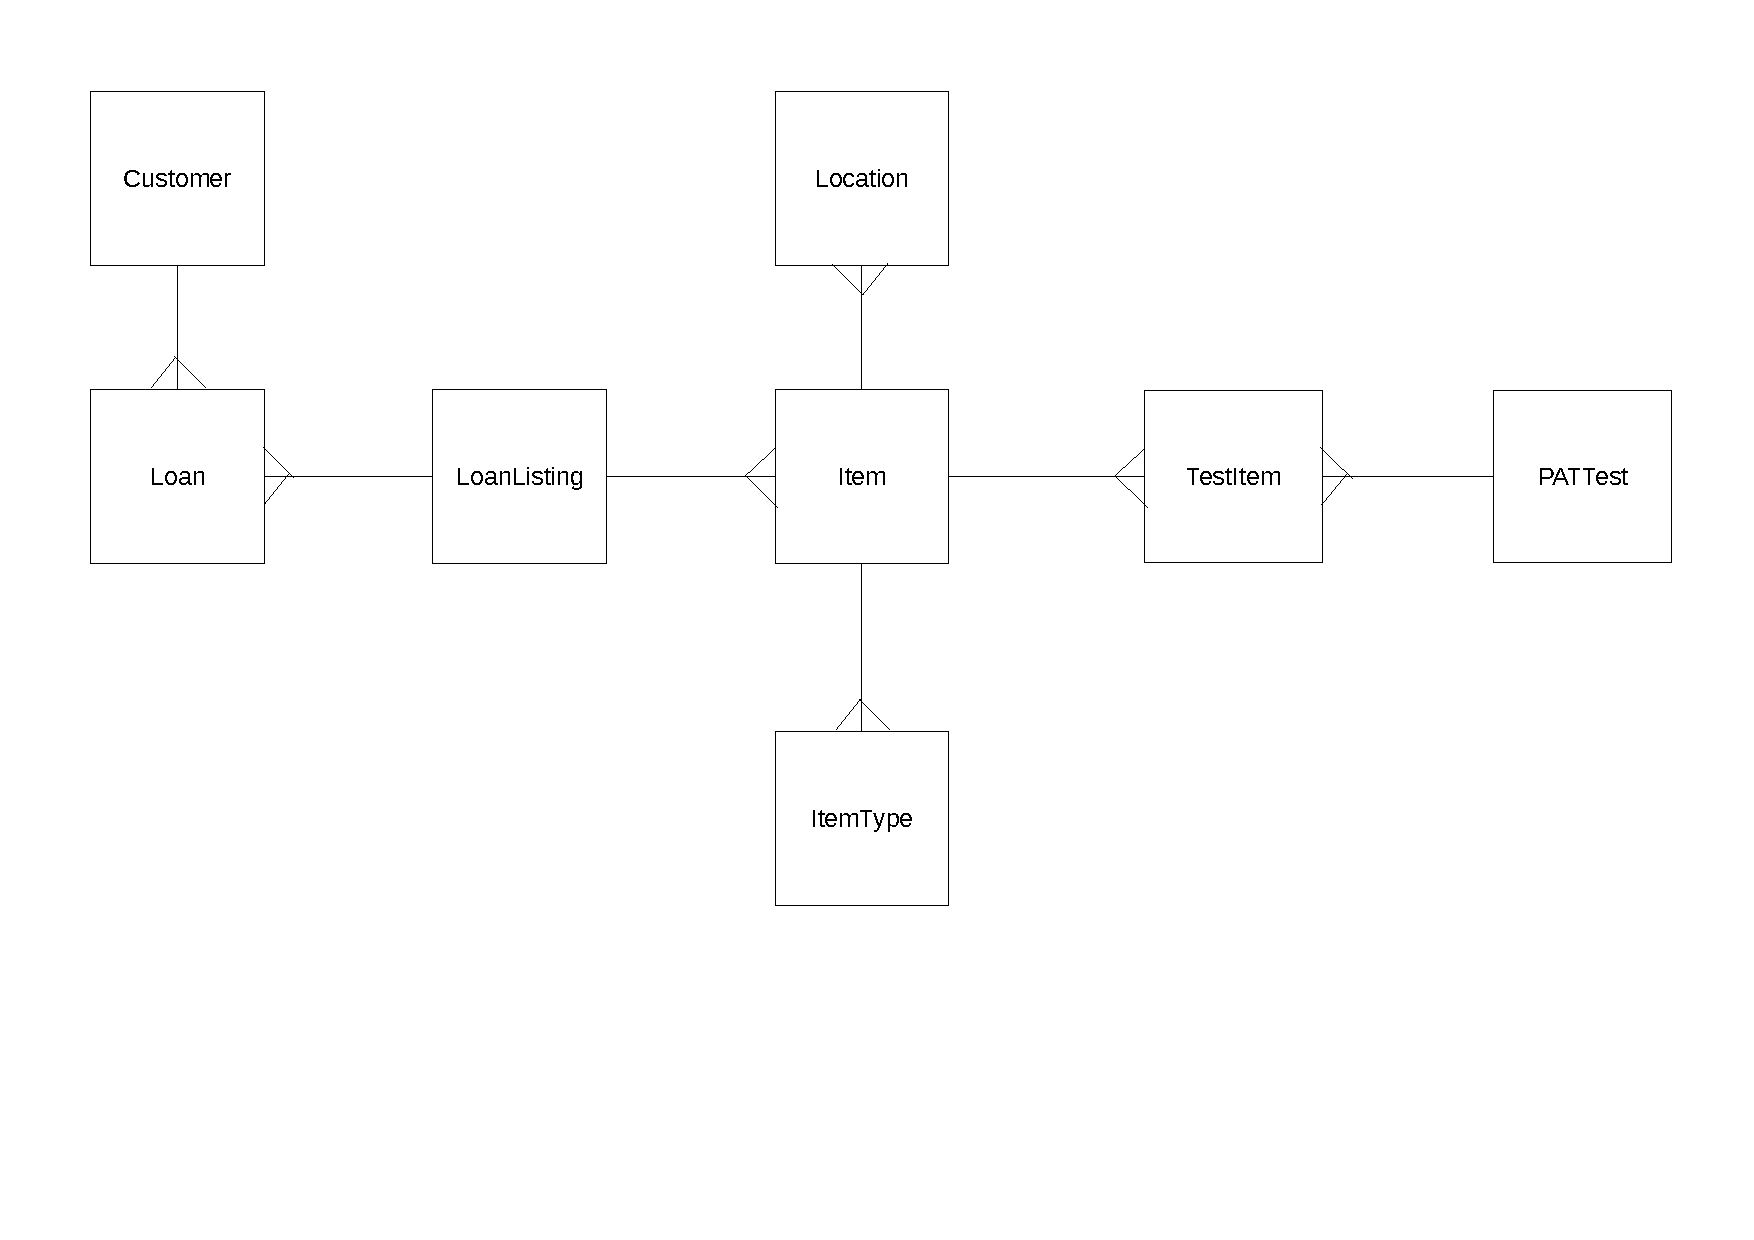
\includegraphics[width=490px]{./Design/Database_Design/Normalisation/ER_Diagrams/ER_Diagram.pdf}}
    \caption{ER Diagrams.} \label{fig:ER Diagrams}
\end{figure}

\end{landscape}

\subsubsection{Entity Descriptions}

\begin{center}
    \begin{tabular}{|c|}
        \hline
        \textbf{Un-Normalised Form(UNF)}\\ \hline
        ItemID\\ \hline
        ItemName\\ \hline
        ItemType\\ \hline
        Location\\ \hline
        Value\\ \hline
        ItemQuantity\\ \hline
        SubTotal\\ \hline
        OnLoan\\ \hline
        LoanID\\ \hline
        LoanQuantity\\ \hline
        LoanRate\\ \hline
        LoanLength\\ \hline
        LoanCost\\ \hline
        CustomerID\\ \hline
        Forename\\ \hline
        Lastname\\ \hline
        Company\\ \hline
        Street\\ \hline
        Town\\ \hline
        PostCode\\ \hline
        MobileNumber\\ \hline
        LandLine\\ \hline
        Email\\ \hline
        PATtestID\\\hline
        TestResult\\ \hline
        TestDate\\ \hline
        ItemDescription\\ \hline
        ItemClass\\ \hline
        FuseRating\\ \hline
        TestUsed\\ \hline
        ProtectiveCondTest\\ \hline
        InsulationTest\\ \hline
        Leakage\\ \hline
    \end{tabular}
\end{center}

\newpage

\subsubsection{1NF to 3NF}

\begin{center}
    \begin{tabular}{|c|c|}
        \hline
        \multicolumn{2}{|c|}{\textbf{First-Normalised Form(1NF)}}\\ \hline
        \multicolumn{2}{|c|}{ }\\ \hline
        \textbf{Non-Repeating} & \textbf{Repeating}\\ \hline
        \underline{ItemID }& \underline{LoanID }\\ \hline
        ItemName & \emph{ItemID} \\ \hline
        ItemType & LoanQuantity \\ \hline
        ItemLocation & LoanRate\\ \hline
        Value & LoanLength \\ \hline
        ItemQuantity & LoanCost \\ \hline
        SubTotalValue & CustomerID \\ \hline
        OnLoan &  Forename \\ \hline
         & Lastname \\ \hline
         & Company \\ \hline
         & Street \\ \hline
         & Town \\ \hline
         & PostCode \\ \hline
         & MobileNumber \\ \hline
         & Landline \\ \hline
         & Email \\ \hline
         & PATtestID \\ \hline
         & TestDate \\ \hline
         & ItemDescription \\ \hline
         & ItemClass \\ \hline
         & FuseRating \\ \hline
         & TestUsed \\ \hline
         & ProtectiveCondTest \\ \hline
         & InsulationTest \\ \hline
         & Leakage  \\ \hline
         & TestResult \\ \hline
    \end{tabular}
\end{center}

\section{Security and Integrity of the System and Data}

\subsection{Security and Integrity of Data}

\subsection{System Security}

\section{Validation}

\section{Testing}

\begin{landscape}
\subsection{Outline Plan}

\begin{center}
    \begin{tabular}{|p{2cm}|p{5cm}|p{5cm}|p{4cm}|}
        \hline
        \textbf{Test Series} & \textbf{Purpose of Test Series} & \textbf{Testing Strategy} & \textbf{Strategy Rationale}\\ \hline
        Example & Example & Example & Example \\ \hline
    \end{tabular}
\end{center}

\subsection{Detailed Plan}

\begin{center}
    \begin{longtable}{|p{1.5cm}|p{2.5cm}|p{2.5cm}|p{2cm}|p{2cm}|p{2cm}|p{2cm}|p{2cm}|}
        \hline
        \textbf{Test Series} & \textbf{Purpose of Test} & \textbf{Test Description} & \textbf{Test Data} & \textbf{Test Data Type (Normal/ Erroneous/ Boundary)} & \textbf{Expected Result} & \textbf{Actual Result} & \textbf{Evidence}\\ \hline
        Example & Example & Example & Example & Example & Example & Example & Example \\ \hline
    \end{longtable}
\end{center}
\end{landscape}
